\chapter{Focusing Provider Attention}

\textbf{Focusing Provider Attention: An Empirical Examination of Incentives and Feedback in Flu Vaccinations.}\footnote{This chapter (and the associated Appendix \ref{app_cc}) has appeared in previously published work under the following citation: Niewoehner, R. J., and Staats, B. R. (2021). Focusing Provider Attention: An Empirical Examination of Incentives and Feedback in Flu Vaccinations. \textit{Management Science}. The chapter is reproduced with permission from the rightsholder, The Institute for Operations Research and the Management Sciences (see \textit{\href{https://marketplace.copyright.com/rs-ui-web/mp/license/4d1e513c-a5c2-48d3-b82a-56891a9baac7/9317d961-3fc3-423f-9eff-01148c7093b6}{here}} for link to license agreement).}
This Chapter is co-authored with Dr. Bradley Staats.

    % Elements of this Chapter  are common to \\
    % \cite{Niewoehner2021}, which is reproduced with permission from the rightsholder: \\
    % The Institute for Operations Research and the Management Sciences (INFORMS) \\ 
    % (see \textit{\href{https://marketplace.copyright.com/rs-ui-web/mp/license/4d1e513c-a5c2-48d3-b82a-56891a9baac7/9317d961-3fc3-423f-9eff-01148c7093b6}{here}} for link to license agreement).

% \begin{center} \rule{6in}{0.01in} \end{center}
% \noindent
%   \textbf{Chapter Abstract:} \\
%   \textbf{Background:} Influenza imposes heavy societal costs through healthcare expenditures, missed days of work, and numerous hospitalizations each year. Considering these costs, the healthcare and behavioral science literature offers suggestions on increasing demand for flu vaccinations. And yet, the adult flu vaccination rate fluctuated between 37\% and 46\% between 2010 and 2019. \\
%  \textbf{Aim:} Although a demand-side approach represents one viable strategy, an operations management approach would also highlight the need to consider a supply-side approach. In this paper, we investigate how to improve clinic vaccination rates by altering provider behavior. \\
%  \textbf{Methodology:} We implement and study a flu vaccine intervention among 145 clinics from 9 different states. This intervention randomly assigned these clinics to a control group or one of two separate treatment arms that received either relative performance feedback or financial incentives.  \\
%  \textbf{Results:} We find clinics that received relative performance feedback outperformed all others: Our intervention led to a 12\% increase in flu shots for this group of clinics. Moreover, we also find clinics in this group exhibit rank response behavior, specifically Last-Place Aversion; in particular, clinics near Last-Place outperform the corresponding control clinics by 23 percentage points.  \\  
%  \textbf{Conclusion:} Overall, we find that clinic-level performance feedback can effectively drive operational improvement. Even a small increase in the US adult flu vaccination rate might confer hundreds of millions of dollars in societal benefits and prevents thousands of hospitalizations. We discuss the implications of our work for healthcare operations theory, healthcare providers, and healthcare administrators. 
% \begin{center} \rule{6in}{0.01in} \end{center}

% \noindent\keywords{Healthcare; Attention; Incentives; Performance Feedback; Empirical Operations } \\

\section{Introduction} 
 Every year influenza significantly impacts millions of people’s health and imposes heavy societal costs through healthcare expenditures, missed days of work, and hundreds of thousands of hospitalizations \citep{Molinari2007,CDC2020_fluBurden}. Consider that as recently as the 2017-18 flu season, the United States Centers for Disease Control and Prevention (CDC) identified extended, epidemic-level mortality due to flu outbreaks \citep{Garten2018}. To prevent these outbreaks, experts maintain that the seasonal flu vaccine “remains the best way to protect” against the flu \citep[p. 544]{Xu2019}, and the majority of US adults accept this fact \citep{NationalFoundationforInfectionsDiseasesNFID2019}. Despite this, and even though the CDC recommends the vaccine for everyone older than 6 months, the adult vaccination rate remained between 37\% and 46\% each season between 2010 and 2019 \citep{CDC2019}.
 
 Given this relatively low compliance rate (compared to full compliance near 100\%), it is not surprising that researchers in public health have focused on increasing demand for flu vaccinations \citep{Brewer2017}. This “demand-side” approach concentrates on increasing patients’ likelihood of seeking the vaccine from their provider. The most successful of these interventions engage patients directly, for example, by getting them to commit to a time \citep{Milkman2011} or scheduling an appointment on their behalf \citep{Chapman2016}. However, success eludes most studies that seek to alter patients’ thoughts and feelings on vaccinations \citep{Brewer2017}. Now, perhaps more than ever, society needs better field studies to identify interventions that work.
 
 Thus, a quandary exists – the high costs of the flu, and the potential implications for other vaccines, demand action while existing approaches for vaccine compliance exhibit significant limitations. Although a demand-side approach might be viable, an operations management approach would also highlight the need to consider the supply-side: Driving compliance by focusing provider attention on vaccine provision. The question of compliance to standards is one that has been explored by the operations field from its earliest years \citep{Taylor1911} through today \citep{Corbett2005,Andritsos2014,Senot2016,Staats2017}. Not only does the supply-side approach include ensuring that sufficient vaccine supply flows smoothly through the supply chain \citep{Deo2009,Cho2010,Arifoglu2012}, but also it highlights the key role that providers play in delivering a service. Healthcare operations frequently focus on how providers shape a service system \citep[e.g.,][]{Tucker2007,Freeman2017} and recent work has explored interventions to alter provider behavior in positive ways \citep{Tsai2015,Song2016,Dai2017,Song2018a}. 
 
 In this paper, we blend work on operational compliance and healthcare operations to investigate how to improve clinic vaccination rates by altering provider behavior. To answer this overarching question, we contrast two intervention mechanisms: Financial incentives and performance feedback. Both supply-side interventions might affect clinic vaccination rates, but which is more effective remains unknown. Finally, we explore one path to altered provider behavior and ask: Among high and poor performing clinics, does a “love of first” or a “fear of last” lead to better outcomes?
 
 To answer these questions, we implement and study a flu vaccine intervention. This experiment launched in August 2018, where 145 clinics from 9 different states were randomly sorted into three distinct groups: (1) a Control group, which received no further intervention; (2) a Ranking group, which only received performance feedback – in the form of rankings – based on clinic flu shot growth; and (3) a Rebate group, which only received financial incentives for clinic flu shot growth. We find that firms receiving relative performance feedback significantly outperform incented (and control) firms. Few studies examine the impact of both treatments at the firm-level, and even these exceptions cannot identify which is more effective. This contributes to a growing body of work that highlights operational performance may be improved more by altering non-monetary factors than monetary factors, in certain situations. In addition, we test for and demonstrate the presence of rank-response behaviors, specifically Last-Place Aversion where clinics near the ranking floor increased their vaccination performance more than others. We believe that we are the first to show that this manifests as a dynamic effect outside of the lab at the firm-level, whereby effort is exerted to move away from last place each week.
 
 Overall, we find that private, relative performance feedback can effectively drive operational change as relative performance feedback led to an 9.8 percentage point increase in flu vaccines. This has important implications for public policy as even just a 1 percentage point increase in the US adult flu vaccination rate could confer \$380 million in societal benefits \citep{White2021}. Even further, by intervening at the clinic level, we do not interfere with providers’ discretion, and thus aim to enable, not hinder, better patient care. Our results are practically relevant for healthcare and also add to the field of people-centric operations whereby workers productively use their discretion to improve operational performance. 

 
\section{Previous Literature \& Hypothesis Development} \label{HD_CC}
 \subsection{Relevant Literature}
 At its core, the flu vaccination problem represents a mismatch between supply and demand. Matching supply to demand is a key tenet of both economics and operations management, and so our study sits at the intersection of the operations, economics, and medical literature. The medical focused literature offers many suggestions for increasing demand for flu vaccinations \citep[see][]{Brewer2017}. The most successful studies introduce prompts compelling employees to specify a time to receive their vaccination at an upcoming on-site clinic \citep{Milkman2011} and utilize opt-out appointment conditions \citep{Chapman2010,Chapman2016}. However, despite their success in changing patient vaccination beliefs, many of these studies lack proof of changing patient vaccination behavior.
	
 Though fewer in number, some medical studies have instead taken a supply-side approach. Effective supply-side strategies might reduce “missed opportunities for vaccination” \citep{Jaca2018} or they might combine supply- and demand-side approaches \citep{Smulian2016}. For example, \cite{Gilkey2014} intervened by offering clinicians an opportunity to consult with an immunization specialist. Two consultations occurred five months apart and revealed: (1) each clinic’s vaccine specific immunization rates, and (2) the average vaccine coverage for that clinic’s county. Generally though, Electronic Health Record (EHR) alerts represent the most common intervention strategy \citep{Fiks2009,Fiks2013,Zimmerman2014,Szilagyi2015,RuffinIV2015,Lin2016,Patel2017}. These EHR alerts prompt clinicians to order vaccinations during patient appointments. Other clinical interventions are frequently added to these alerts. For example, in their study of pediatric human papillomavirus (HPV) rates, \cite{Fiks2013} combined EHR alerts, clinician education, and 3 quarterly consultations evaluating each clinic’s vaccination rates. In \cite{Zimmerman2014} study of pediatric flu vaccinations, the authors added 15 protocols on top of EHR alerts, including patient reminders, office posters, and even paying staff for a mid-season training session. Indeed, some of these studies improved outcomes, but such multi-pronged approaches struggle to objectively identify direct mechanisms \textit{ceteris paribus}. Thus, we can build on these supply-side efforts by teasing out specific effects.
	
 Which of these intervention strategies would be most effective in our setting, given what we know from other streams of literature? Some of these strategies evaluate various forms of provider performance feedback (training, consultations, audits, etc.) which occur outside a patient encounter, unlike EHR alerts. Performance feedback studies are common in the economics literature \citep[see reviews in][]{Dechenaux2015,Schnieder2019} and performance feedback frequently induces positive outcomes \citep{Casas-Arce2009,Azmat2010,Blanes-i-Vidal2011,Delfgaauw2013,Song2018a}. Thus, performance feedback seems promising given the common support in both literatures.
	
 And yet, despite the overlap, many of these studies carry significant limitations. On the medical side, endemic issues include small sample sizes, invalid controls, and poor experimental design \citep[p. 1585 in][]{Smulian2016}; moreover, these studies largely ignore adult vaccinations. But perhaps most troubling for these studies is the reliance on EHR alerts: These alerts accompany growing skepticism within the medical community because of the increasing prevalence of “alert fatigue” among providers \citep{Peterson2001}. This is especially concerning when up to 96\% of these alerts may end up overridden or ignored \citep{VanDerSijs2006}. Other opportunities exist to build on the economics literature, given the lack of randomized field studies and the reliance on behavioral lab experiments. Furthermore, nearly all studies of performance feedback include elements of performance pay such that the effect of each cannot be separated \citep[e.g.,][]{Delfgaauw2014}. \cite{Schnieder2019} differentiates between such tournament incentives and relative performance feedback, or RPF, which is given separate of financial outcomes. Thus, the call remains for robust, generalizable vaccine interventions which reduce the risk of real-time, technological interference between provider and patient while still allowing unambiguous identification of a treatment’s outcome.
	
 Given this call, an operations framework can effectively address these limitations. First, this framework acknowledges the need for researchers who “situate their work clearly in the [actual] context” under study \citep[p.121]{Ibanez2019a}. This approach demands a relevant context and proper experimental design to achieve robust managerial implications. Second, operations management research acknowledges the important role of individual discretion in operational outcomes \citep[e.g.,][]{VanDonselaar2010,Campbell2011,Kim2015,Phillips2015}. Though these outcomes are sometimes negative \citep{Ibanez2017,Ibanez2019}, they are frequently positive \citep{Freeman2017,Song2018a}. But since technological interference (such as EHR alerts) hinders discretion indiscriminately, we ask, “How do we keep the discretion we want?” The answer: Deliberate system design, which can transform problematic deviance into productive discretion by focusing attention on the outcome of interest. For instance, we know even a small attention cue can encourage physicians to improve their processes \citep{Song2018a,Kim2020}. Separate from performance feedback or tournament incentives, piece-rate incentives present another common element of system design \citep{Prendergast1999,Lazear2018}. Studying each in isolation allows us to tease out the advantages of RPF over tournament incentives and further the literature in this area. 
 
 Thus, at the intersection of these three streams of literature, we compare two, separate attention cues: (1) piece-rate incentives; and (2) relative performance feedback. We study how both cues may impact providers’ discretion by focusing their attention on supplying flu vaccinations to their patients and address the concerns above. First, we randomly assign clinics to treatment and control. Second, our study includes more clinics with more geographic diversity: our sample of 145 clinics represent 9 states and 77 counties. Third, we isolate the incentive and feedback treatments to compare the effect of each. Finally, unlike the medical studies, we intervene at the clinic level rather than the provider level. This approach clarifies the individual response within the context of a firm while simultaneously eliminating any technological hindrance of patient care. We proceed to specify the current flu vaccination problem and propose strategies to improve clinic vaccination outcomes.  

 \subsection{Improving Vaccination Outcomes}
 From a supply-side perspective, the greatest opportunity for vaccination improvement surrounds the “last mile” problem: The administration of the shot. Many other supply issues have already been addressed. For example, the CDC now stockpiles a supply of flu vaccinations in the event of unexpected shortages. Additionally, manufacturers mitigate under-ordering with buy-back contracts \citep[e.g.,][]{Pasternack1985}. And since previous operations literature proposed improvements for the flu vaccine supply chain \citep{Deo2009,Cho2010,Arifoglu2012}, the Food and Drug Administration has not noted a significant flu vaccine shortage in the last 5 years \citep{FDA2020}. 
 
 Despite the medical community’s efforts to increase demand and guarantee supply, the flu vaccination rate in the US has changed little in recent years. Adult vaccination rates for flu seasons 2010-11 through 2018-19 fluctuated between 37.1\% and 45.3\% \citep{CDC2019}. Patient rejection cannot explain this stagnation. Consider that under any health insurance plan, flu vaccinations are covered at zero patient cost in compliance with the Affordable Care Act. Furthermore, the general rate of vaccine rejection remains stable and low at less than 2\% \citep{Brewer2017}. On the contrary, \cite{Patel2017} find that more than 99\% of patients accept the flu vaccine when providers recommend it. Thus, patients rarely avoid or refuse recommended vaccines. Instead, it is much more likely that providers simply do not offer as many flu vaccines as they should. 
 
 Why then are providers not offering more flu vaccinations? One possible explanation is that providers experience severe demands on their time and attention. To follow all patient care guidelines, estimates say primary care physicians need to spend at least 7 hours on prevention \citep{Yarnall2003} and 11 hours on treatment \citep{Ostbye2005} each day. In a survey of more than 9,000 physicians, 80\% reported over or at-capacity utilization, and 78\% reported regularly experiencing feelings of burnout \citep{ThePhysiciansFoundation2018}. These physicians have numerous, competing, demands on their attention.
 
 Given these demands, how might clinics design their system to focus provider attention? Simple interventions might suffice. Financial incentives “lead to more effort and higher performance” \citep[p. 191]{Gneezy2011}, but firms might also consider non-financial incentives to influence healthcare provider behavior \citep{Song2016,Jaeker2019}. Performance feedback can change the “reference structure” within a firm and alter individual output \citep{Roels2014}. Vaccination behavior might also improve with a simple attention cue that requires a provider to actively choose instead of relying on passive workflow \citep{Patel2017}. Or consider that training can highlight areas for system-level vaccine improvement \citep{Gilkey2014}. From the behavioral perspective of a firm, the operational structure channels attention by prioritizing decision makers’ tasks \citep{Simon1947,Hayes1988,Ocasio1997,Ocasio2018}, and system design informs this structure.
 
 Since system design focuses attention within a firm, how can we influence firm-level design choices within a network of firms? To achieve large-scale improvement, independent clinics will have to unilaterally address their flu vaccinations. But firms are composed of individuals, so team- and firm-based incentives may also yield positive outcomes, despite the temptation to freeride \citep{Bandiera2007,Friebel2017}. However, “the number of existing empirical studies providing causal estimates on the effects of team incentives is still quite small” \citep[p. 10]{Delfgaauw2020a}, and even less is known about group-based feedback  \citep[e.g.,][]{Delfgaauw2013}. Given (1) the importance of flu vaccinations, and (2) the fact that no single clinic can affect broad improvement – new research is critical to plugging this gap. 
 
 Accordingly, we test two firm-level factors: Financial incentives and relative performance feedback. We intervene at the clinic level in a network of independent healthcare clinics: A clinic’s management team receives the financial incentives and only the management team learns their vaccination performance. As a result, the clinic managers have full discretion to redirect incentives and share feedback with frontline providers. Our work sheds light on the role and effectiveness of firm-level interventions and how such interventions might be further leveraged to address large-scale issues. We propose that providing financial incentives and relative performance feedback to a firm will positively affect that firm’s decision-making processes, leading to an increase in flu shots.
 
 \medskip \noindent
 \begin{tabularx} {\linewidth}{ r X }
    \textbf{Hypothesis 1a:} & \textit{Treated clinics who receive financial incentives for reaching growth thresholds will show greater Year-over-Year growth in flu shots administered than the respective control clinics.} \\
    \textbf{Hypothesis 1b:} & \textit{Treated clinics who receive performance feedback relative to other clinics in the same treatment group will show greater Year-over-Year growth in flu shots administered than the respective control clinics.}
 \end{tabularx}   %\medskip 
 
 \subsection{More Effective: Incentives or Feedback?}
 A follow-up question is which treatment is most effective in driving flu shot growth: Financial incentives or performance feedback? Although financial incentives can backfire, such as when they “crowd-out” intrinsic motivation \citep[e.g.,][]{Deci1971,Fehr2000,Gneezy2011,Staats2017,Lazear2018}, the research consensus is that paying for performance induces better performance. Conversely, the conclusions from the performance feedback literature are less clear. In fact, similar studies frequently generate contrasting results \citep[as discussed in][]{Dechenaux2015}. For example, some studies find a positive effect with the provision of RPF \citep[e.g.,][]{Casas-Arce2009,Azmat2010,Blanes-i-Vidal2011,Delfgaauw2013,Song2018a}). Other studies find negative effects \citep[e.g.,][]{Barankay2012,Bandiera2013,Ashraf2014}, positive and negative effects \citep[e.g.,][]{Blader2016}, or no effect \citep[e.g.,][]{Delfgaauw2014}. The conditions under which RPF has a positive, negative, or null effect are not well understood.
 
 The question of which effect will dominate is eventually an empirical one: Of the studies we examined, only \cite{Delfgaauw2013} has a multi-firm setup where the effect of incentives and feedback can be compared; however, the authors cannot statistically identify which treatment has a greater effect. Nevertheless, because of (1) the consistent conclusions of the incentives literature; (2) the low likelihood of crowding-out due to the existing financial motivation to administer flu shots; and (3) the mixed results from the feedback literature; we propose that clinics in a financially incentivized treatment will outperform clinics who are provided with performance feedback.
 
 \medskip \noindent
 \begin{tabularx} {\linewidth}{ r X }
    \textbf{Hypothesis 2:} & \textit{Treated clinics who receive financial incentives for reaching growth thresholds will show greater Year-over-Year growth in flu shots administered than clinics who receive relative performance feedback.} \\
 \end{tabularx}   %\medskip 
 
 \subsection{Response to Performance Feedback}
 Within the ranking condition, we expect distinct behavioral responses to differing ranks. Relative position really matters. People have an innate desire to evaluate their own capabilities, and comparative feedback enhances one’s ability to accurately evaluate their own performance \citep{Festinger1954}. \cite{Kuziemko2014} recall the childhood fear of being “picked last in gym class” in their seminal study of Last-Place Aversion. In the end, better or worse ranks may lead to different responses to performance feedback.
 
 Despite this fact, most literature ignores this effect. In addition to \cite{Kuziemko2014}, another exception is \cite{Gill2019}, where the authors experimentally characterize a U-shaped rank response function. Their participants demonstrated both “First-Place Loving” (FPL) and “Last-Place Aversion” (LPA) behaviors: Participants ranked near the top and the bottom exerted increased their effort, while modestly ranked participants scaled back their effort. Even still, both \cite{Kuziemko2014} and \cite{Gill2019} study these behaviors among individuals in the lab. Will these results generalize, since “in the real world, the concept of last place is far less well defined” \citep[][p. 107]{Kuziemko2014}? Interestingly, \cite{Buell2021} shows that last place can change real-world, consumer behavior as (1) customers at the end of a supermarket queue are more likely to abandon and (2) the effect disappears when no longer last. 
 
 Building on prior work, we highlight the need to consider rank response in real contexts at the firm-level with flexible definitions of first and last place. We investigate whether individuals exert discretion (giving more flu vaccinations) in response to rank information. In addition, we further relax the definitions of first and last place, where an aversion to last place, for example, may manifest when ranked within some range of the extreme. In so doing, our work is related to \cite{Song2018a} who find that when productivity feedback is public (names are known), physicians ranked near the bottom improve the most. We examine the dynamic impact of rankings, however, and this is a key difference. \cite{Song2018a} study a context where stars or laggards stay constant, and so they fix their top and bottom performers as a function of the pre-intervention performance. In contrast, we study clinics who move in and out of relative rankings instead of individuals who maintain their relative position. The change in our firm-level rankings provides the opportunity to study the dynamic effect on performance. In line with prior work, we propose rank-response behaviors will be evident among both high and low performers. 

 \medskip \noindent
 \begin{tabularx} {\linewidth}{ r X }
    \textbf{Hypothesis 3:} & \textit{Clinics ranked near the top will increase their vaccination rate to maintain a position amongst high-performing clinics.} \\
    \textbf{Hypothesis 4:} & \textit{Clinics ranked near the bottom will increase their vaccination rate to move away from other poor-performing clinics.}
 \end{tabularx}   %\medskip 
 
\section{Experimental Setup \& Empirical Approach} \label{empirics}
 \subsection{Company Setting}
 We test our hypotheses with data provided to us by VaxCare, a vaccine management company. VaxCare partners with health care clinics to manage vaccination logistics. This includes ordering vaccines from the manufacturer, managing clinic inventory, and billing the payer. VaxCare partner clinics vary in size, from smaller, regional clinics to larger networks of clinics. Clinical staff for these partners include physicians (median: 2 per clinic), nurses, medical assistants (MA), and office staff.
 
 Prior to administering a vaccination, providers scan each shot into VaxCare’s technology hub and digitally assign that shot to a patient. Though vaccinations must be ordered by a physician, they are usually administered by a nurse or MA. Some physicians implement “standing orders” in their office so shots can be given without requiring a physician signature for every patient. Such orders for flu shots empower staff to pursue the CDC’s recommendation to vaccinate everyone for flu. VaxCare’s flu vaccination trends are similar between years: Some shots are given in early August, with a peak in October and then trend downward as the year concludes. For the purposes of this paper, we define the flu vaccination season as 1 August through 31 December; 95\% of VaxCare’s flu shots occur in this window. 

 \subsection{Pilot Study in 2017}
 In August 2017, VaxCare launched a pilot study to test whether the introduction of financial incentives and relative performance feedback positively impacted flu shots. A VaxCare program director recruited 101 Florida clinics to participate during the 2017 flu vaccination season. Program feedback included clinic progress toward an incentive tier and a performance ranking relative to other clinics in the program.
 
 The results from the pilot were positive: Clinics in the study administered 33.5\% more flu shots than other Florida clinics outside the study. However, we could not tell whether the difference was driven by the financial incentives, performance feedback, or some combination of both. These findings identified the need to execute a randomized field experiment. The design of the field experiment, especially the consideration criteria, were directly informed by our analysis of the pilot study. Please see the Appendix (Section \ref{app_cc_pilot}) for a complete description of the setup and results from the pilot study.

 \subsection{Compliance Care 2018: Setup, Randomization, and Response} \label{cc_setup}
 Informed by the outcomes of the pilot study, study clinics were identified and randomly assigned by state to one of three arms. Compliance Care 2018 officially launched in August 2018 and included 145 clinics from 9 states. Section \ref{app_exp_design} details our experimental design and clinic consideration criteria, as well as the treatment specifics. Between clinic recruitment and the start of the study, five clinics terminated their VaxCare partnership. After randomization, we test for balance across the treatment and control groups to validate our randomization efforts (see full discussion in Section \ref{app_cc_sens}).
 
 After recruitment, no further action was taken with the Control clinics; this setup simulates the typical relationship between VaxCare and a partner clinic. The Rebate clinics received tiered incentive thresholds with rebates of \$1, \$2, and \$3 per shot awarded for achieving the targets set at 10\%, 15\%, and 20\% Year-over-Year flu shot growth. The Ranking clinics were provided with weekly rankings based on their overall Year-over-Year percentage growth versus other Ranking clinics. VaxCare generated the clinic rankings based on percent growth in 2018 versus the same week in 2017. For example, if a clinic administered 110 shots by week 40 in 2018 and 100 shots by week 40 in 2017, their respective growth would be 10\% in week 40 2018 and they would be ranked against other clinics using this metric. The treated clinics received an email each week. Ranking clinics received anonymous relative rankings, while Rebate clinics were given their percent growth and progress towards the incentive tiers. 
 
 How might these clinics respond to this information? During recruitment, clinics generally identified an office administrator to receive the Compliance Care emails from VaxCare. Herein lies a key contribution of our work: Our intervention ends with this email. Clinic response might vary by clinic. For example, some clinics might implement standing orders to reduce administrative barriers to immunization. The rebates were given to the clinic at the end of the season, and so these clinics might decide in advance to allocate the rebates to the frontline staff. After our study, we learned that the rankings were frequently shared with the entire office in a weekly staff meeting. In any case, we took no further action. Our results highlight the effect of a high-level intervention, where firm-level information might, or might not, trickle down to the individual provider. This approach delegates patient care and vaccination to the clinician, ultimately preserving their discretion to care for their patients. Furthermore, our study contributes to the limited literature surrounding team- or firm-level incentives and feedback. 
 
 \subsection{Empirical Analysis Strategy} \label{emp_strat}
 To evaluate the overall outcome of the experiment, expressed in Hypotheses 1a, 1b, and 2, we apply a \textit{difference-in-differences} approach. Specifically, we compare the difference for the treated clinics (Ranking/Rebate) between 2017 and 2018 to the difference for the Control clinics between 2017 and 2018. The resulting outcome is the average treatment effect (the effect of the experiment on the average outcome of clinic shots). This setup is in line with \cite{Bertrand2004} and \cite{Wing2018}. To evaluate this longitudinal regression, we utilize a Random Effects framework \citep[as defined in][]{Wooldridge2010}. Specifically, we assume any unobserved, individual effect for a clinic is independent of the treatment, which is justified by random assignment to treatment. Additionally, given the results of our randomization check in Section \ref{app_cc_sens}, we exclude four clinics without “common support” when testing these hypotheses; robustness checks for these exclusions can be found in the Appendix (Section \ref{app_cc_sens}).
 
 For Hypotheses 3 and 4, we evaluate the behavioral patterns only within the Ranking clinics. Here, we do not assume independence between unobserved clinic factors and observed covariates (specifically clinic ranking over week). As such, we utilize a Fixed Effects framework \citep[][]{Wooldridge2010} and construct independent variables to test for behavioral patterns.
 
 In all our regressions, we cluster the errors at the clinic level to correct for serial correlation and heteroskedasticity within clinics, in-line with the clustering discussion in \cite{Bertrand2004}. 
 
 \subsection{Independent Variables}
 To test Hypotheses 1a, 1b, and 2, we compare outcomes between 2017 and 2018 using a multi-level factor variable which contains a level for each group (Control/Ranking/Rebate). The resulting output measures the difference between the groups in 2018 during Compliance Care. To test Hypotheses 3 and 4, in line with \cite{Gill2019}, we characterize the full rank response function. This function estimates a clinic’s response to specific rank feedback. To do this, we introduce linear and quadratic variables for ‘Rank.’ Thus, without imposing any definitions on first or last place, we test whether the extremes respond to ranking information differently. As the email update arrived at the end of the week, we lag these variables by one week.
 
 \subsection{Dependent Variables and Model Characterization}
 Our primary outcome of interest is the difference in clinic vaccinations between the treatment and control groups from 2017 (before Compliance Care 2018) to 2018. We want to know if clinics are increasing the number of vaccinations each season in response to the feedback given through the program. To imitate the weekly update emails provided by VaxCare, we have aggregated the data and observed the rate (shots per season) change by week. This period is long enough to make sure that clinics can examine the feedback, but still short enough to capture intertemporal differences. 
 
 \subsubsection{Clinic Flu Shot Percent Growth} \label{emp_spec_pctGrowth}
 To evaluate the outcome of Compliance Care, we implement a general measure of clinic shot performance by calculating the cumulative weekly percent growth of clinics in 2018 over total shots given in 2017. For example, 165 shots given by Week 50 in 2018 would represent 10\% growth from 150 shots given in 2017. This metric also captures differences in clinic size and capacity by measuring growth relative to a clinic’s own performance in 2017. This specification evaluates cumulative percent growth (PercentGrowth) difference ($\beta_1$) between the treated and control clinics (TreatmentGroup) for clinic $i$ in week $t$ while clustering the errors at the clinic level. To allow for changing patient volume and state specific effects, we include a control for patient count (PatientCount) and a state fixed effect (ClinicState). The idiosyncratic shocks which we have not controlled for are captured in $\epsilon$. The Appendix (Section \ref{app_cc_alt_dv}) presents an alternate dependent variable using Cumulative Shots per Patient-Population.
  \begin{equation} %\begin{split} %\end{split} 
       PercentGrowth_{it} = \beta_0 + \beta_1 TreatmentGroup_i + ClinicState_i + PatientCount_i + \epsilon_{it} 
  \end{equation}
 
 \subsubsection{Shots per Patient-Population, by Week}
 To test for the presence of rank response behaviors (FPL/LPA) in the Ranking clinics, we implement a Shots per Patient-Population variable to focus on weekly shots administered. This variable is constructed by taking a clinic’s count of shots given each week and dividing by a clinic’s total number of patients seen for any reason during the vaccination season. This variable enables clinic to clinic flu shot comparison by normalizing by patient volume. Instead of a cumulative outcome, this variable evaluates how a Ranking clinic changes their vaccination behavior in response to their ranking information. 
 \begin{equation} \label{rank_resp} %\begin{split} %\end{split} 
       WeekSPP_{it} = \lambda_0 + \lambda_1 Rank_{i,t-1} + \lambda_2 (Rank_{i,t-1})^2 + Week_t + Clinic_i + \epsilon_{it}
 \end{equation} 
 
 Per Section \ref{emp_strat}, we evaluate this specification using a Fixed-Effects framework. The outcome variable of interest is the shot rate as a ratio of clinic patient-population (weekly shots per patient-population, $WeekSPP$). The Rank variable takes the discrete rank each clinic receives. Like \cite{Gill2019}, to capture the response to the ranking information, we normalize the average value of the rank response to zero for all 46 clinic-rankings, i.e., we constrain $ \Sigma^{46}_{j=1} \lambda_{1,Rank j} + \lambda_{2,Rank j} = 0$. We lag these variables by one week to account for the delayed impact of feedback on behavior, but our results are robust to alternate lags. The Week fixed effect controls for the weekly trend in administering flu shots.
 
\section{Results} \label{Results_CC}
 \subsection{Model-Free Evidence}
 140 clinics started the flu vaccination season in the following groups: Rebate (N = 48), Ranking (N = 46), and Control (N = 46).  The Compliance Care results for each group can be seen in Figure \ref{fig:model_free_cc}. We note the following. First, all groups show an increase in shots administered during Compliance Care. Second, the Ranking group shows the largest growth. Finally, the Rebate group grew slightly more than the Control group (3.2\% versus 2.3\% percent), but well less than the Ranking group. This supports Hypothesis 1a and 1b but contradicts Hypothesis 2. We proceed to test the statistical significance of these findings.
 
 \begin{figure}[htbp]
     \centering
     \caption{Cumulative Flu Shots Administered Before (2017) and During (2018) Experiment} %\medskip
     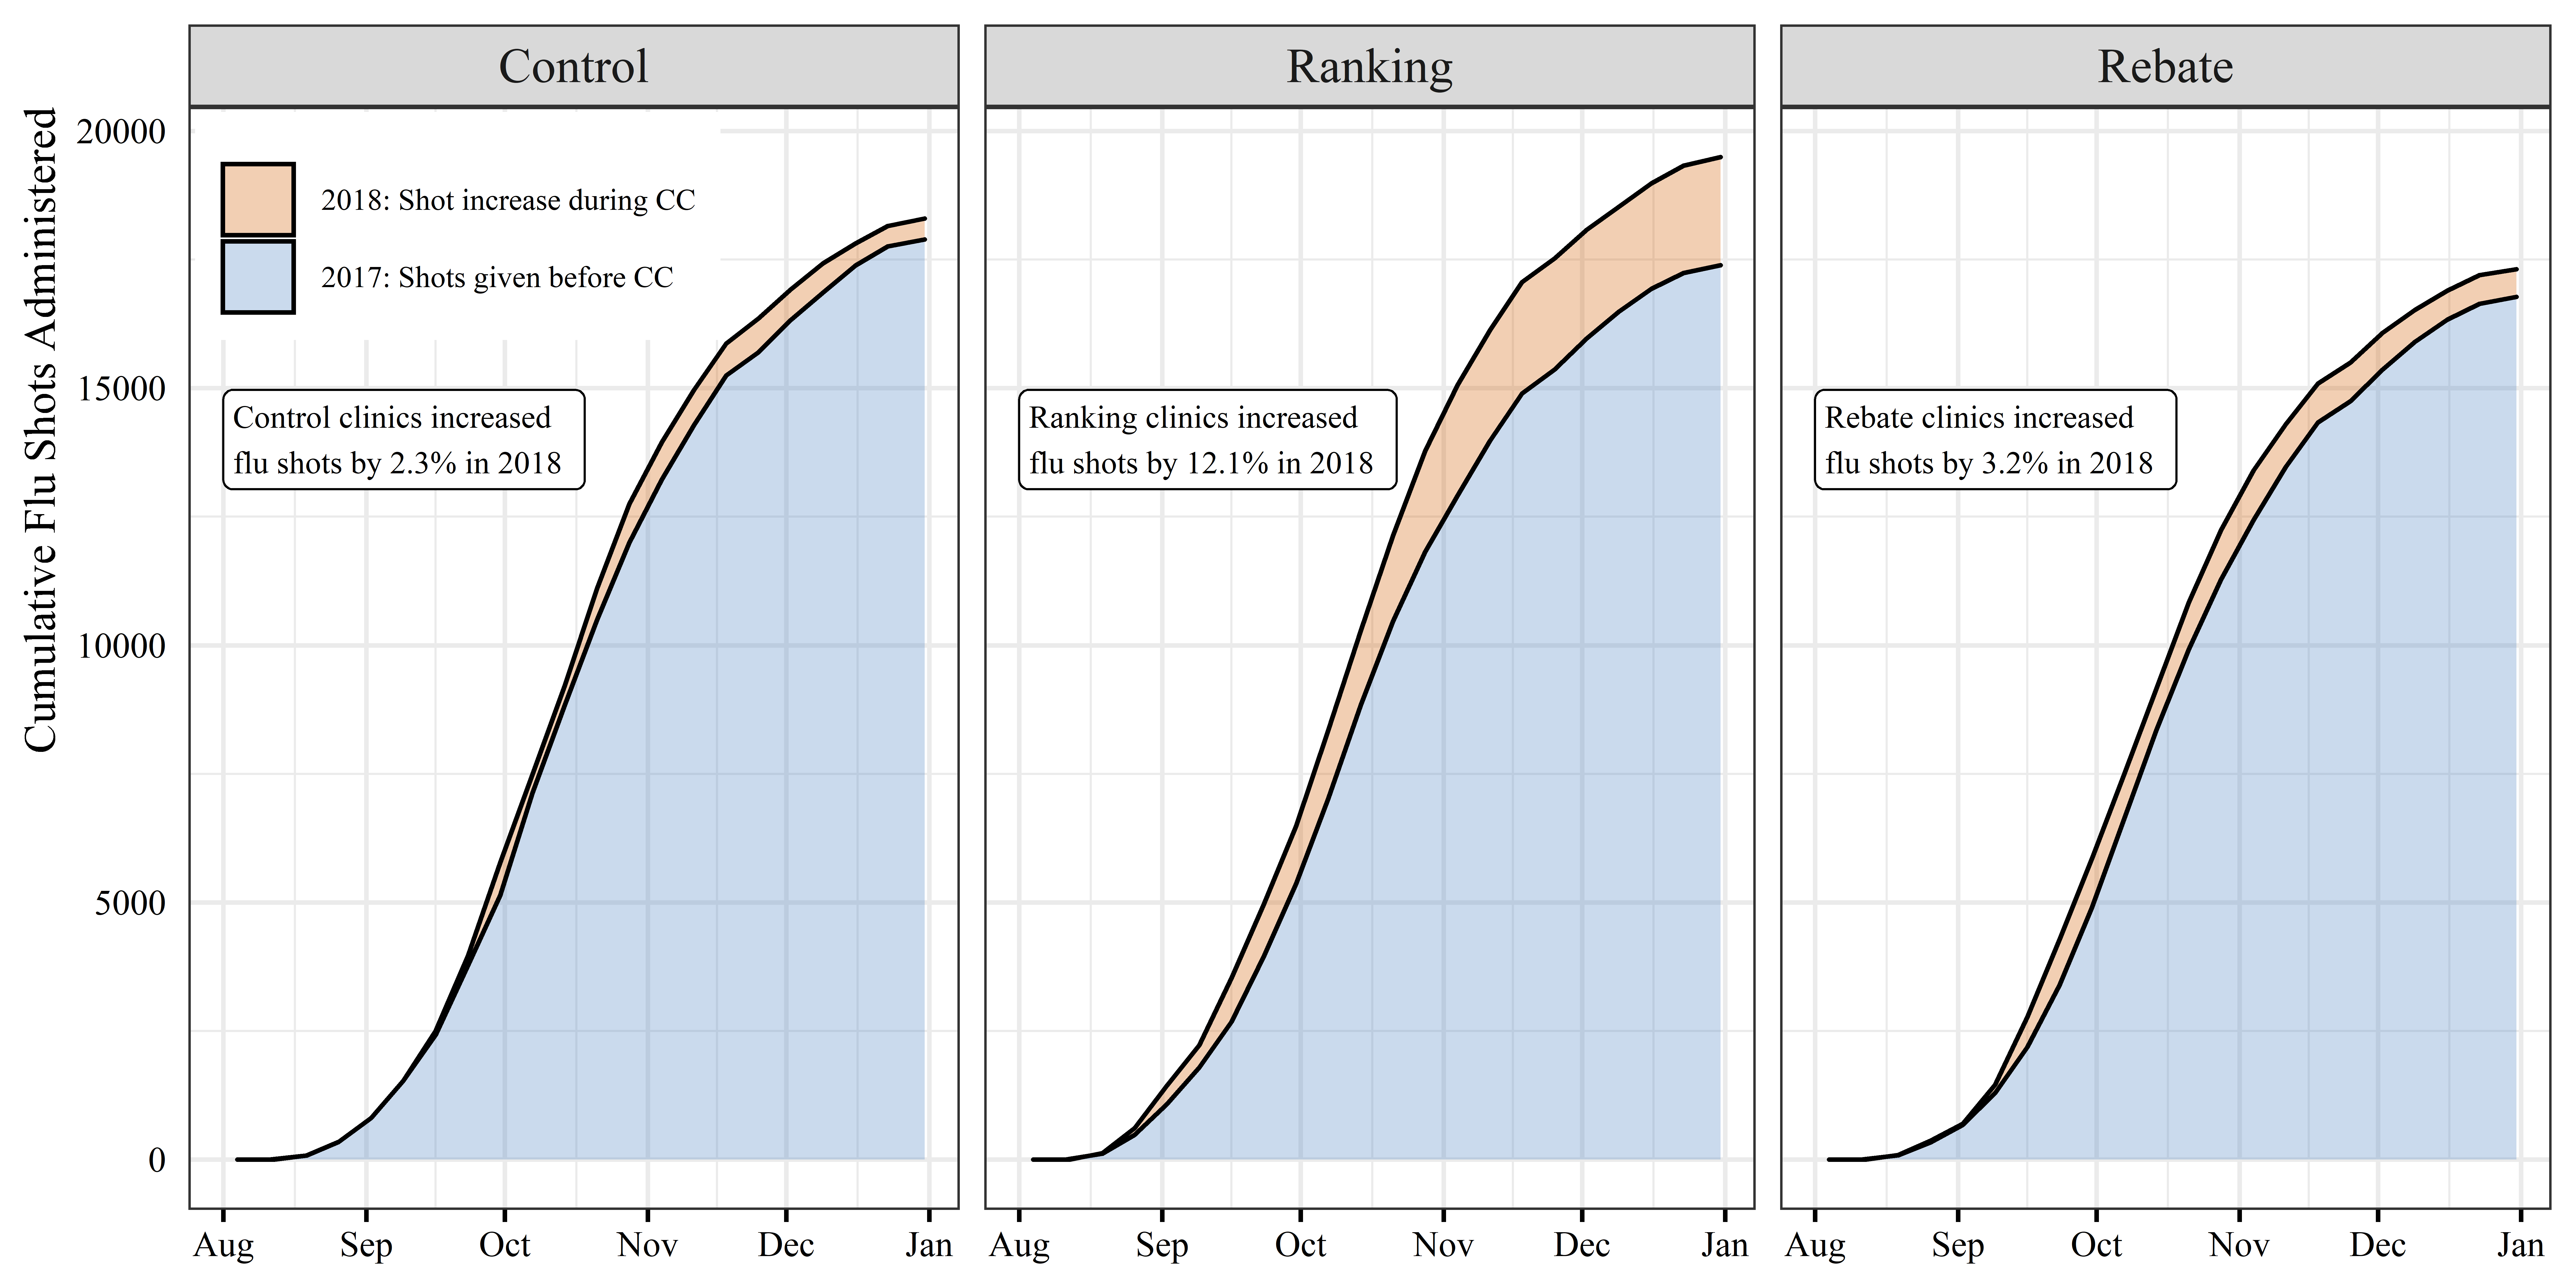
\includegraphics[scale=.75]{Figures/CC/CC_outcome_Fig1_color.png}     
     \label{fig:model_free_cc}
    %  \floatfoot{\textit{Note:} These are some figure notes... }
 \end{figure} 
 
 \subsection{Treatment Effect - Clinic Percent Growth} \label{cc_res_pctGrowth}
 We first examine clinic flu shot percent growth during Compliance Care. For the statistical models that compare clinics from different groups, the most conservative approach is to exclude clinics without common support (N = 136, per Section \ref{app_cc_sens}). Taking the control as the base category, Table \ref{tab:teffect} reveals a statistically significant difference between the Ranking and Control clinics ($p < 0.05$). On average, the Ranking clinics grew their vaccines by 8.3\% more than the Control clinics while the Rebate clinics show no meaningful difference. Thus, we see support for Hypothesis 1b, but not Hypothesis 1a. These results carry through with an alternate dependent variable (Section \ref{app_cc_alt_dv}). One other concern we address: Perhaps Compliance Care emails remind clinics to vaccinate – thus driving our effect. However, both the rebate and feedback conditions received emails, and as discussed next, a significant performance gap exists between the two. We proceed to compare the treated clinic outcomes.
 
  \begin{table}[htbp]
  \resizebox{.5\textwidth}{!}{ 
  \begin{threeparttable}[t]
   \centering
   \caption{Effect of Compliance Care on Clinic Flu Shot Percent Growth}
    \begin{tabular}{lc}
          & (1) \\
          & \textbf{Percent Growth} \\
          & \\
    Ranking (Post-Treatment) & 0.0833** \\
          & (0.0406) \\
    Rebate (Post-Treatment) & 0.00219 \\
          & (0.0399) \\
          & \\
    Observations & 2,720 \\
    \# clinics & 136 \\
    \end{tabular}%
    \medskip
    \begin{tablenotes}
      \footnotesize
      \item \textbf{Table Note:} Robust standard errors, clustered by clinic, in parentheses. Model also includes clinic patient count and clinic state fixed effects. 
      \item (*** $p < 0.01$, ** $p < 0.05$, + $p < 0.1$)
    \end{tablenotes}
  \label{tab:teffect}
  \end{threeparttable} }
 \end{table}
 
 \subsection{Comparison between Ranking and Rebate Groups} \label{cc_res_comp}
 We expected the Rebate group to outperform all others. Instead, the results in Figure \ref{fig:model_free_cc} and Table \ref{tab:teffect} indicate that the Ranking group, who only received performance feedback, outperformed the Control and the incented Rebate group. To test for this, we performed Wald tests on the Table \ref{tab:teffect} coefficients to check whether (1) the Rebate clinics outperformed the Ranking clinics ($H_0: \beta_{1,rebate} >= \beta_{1,ranking}$) and whether (2) the Rebate clinics performed the same as the Ranking clinics ($H_0: \beta_{1,rebate} = \beta_{1,ranking}$). Both tests reject the null hypothesis ($p < 0.05$). Given the results of these tests, we conclude that the Rebate group did not outperform the Ranking group and instead the Ranking group outperformed the Rebate group by a statistically significant margin. Thus, we reject Hypothesis 2 in all cases. We next evaluate the effect of performance feedback within the Ranking clinics. 
 
 \subsection{Rank Response Behavior} \label{cc_res_rankResp}
 During Compliance Care, VaxCare provided relative performance feedback to the clinics in the Ranking group. Each clinic identified at least one staff member to review and share this feedback with the rest of the clinic. As individuals within a firm coalesce around a common response, together they may alter the direction of the firm. Specification \ref{rank_resp} captures clinic response to their previous ranking (Table \ref{tab:rank_effect}, Column 1). 
 
 We observe statistically significant coefficients ($p < 0.01$) for both the linear and quadratic effect of the previous week’s rank. Figure \ref{fig:rank_resp} details the rank response function for each rank generated by these coefficients ($\lambda_1,\lambda_2$) after normalizing the average of these values to zero. This figure illustrates that being ranked last (Rank 46) in the previous week results in about a 2.5\% increase in shots per patient-population this week. In contrast, being ranked first correlates with a 0.8\% increase while being ranked twentieth correlates with a 1.0\% decrease in shots per patient-population. Even with clinic-level feedback, the response to being ranked near last strongly indicates the presence of Last-Place Aversion. We proceed to test the robustness of this finding.

  \begin{table}[p]
  \resizebox{.6\textwidth}{!}{ 
  \begin{threeparttable}[t]
   \centering
   \caption{The Effect of Rank on Weekly Shots per Patient-Population}
    \begin{tabular}{lcc}
          & (1)   & (2) \\
          & \textbf{WeekSPP} & \textbf{WeekSPP} \\
    Clinic Group & Ranking & Ranking \\
    Econometric Model & Specification 2 & Specification 3 \\
          &       &  \\
    Rank, previous week ($\lambda_1$) & -0.00209*** & - \\
          & (0.000648) & - \\
    Rank$^2$, previous week ($\lambda_2$) & 5.34e-05*** & - \\
          & (1.36e-05) & - \\
    Low Flag = 1 if Rank $\in$ & -     & [42,46] \\
    Coeff.: Low Rank ($\pi_1$) & -     & 0.0273*** \\
          & -     & (0.00767) \\
    High Flag = 1 if Rank $\in$ & -     & [1,5] \\
    Coeff.: High Rank ($\pi_2$) & -     & 0.00461 \\
          & -     & (0.00572) \\
          &       &  \\
    Observations & 792   & 792 \\
    \# clinics & 46    & 46 \\
    \end{tabular}%
    \medskip
    \begin{tablenotes}
      \footnotesize
      \item \textbf{Table Note:} Robust standard errors, clustered by clinic, in parentheses. Both models include week fixed effects for all Ranking clinics who started the vaccination season as VaxCare partners. The linear term in Specification 2 ($\lambda_1$) allows a clinic with a change in rank to either increase or decrease their effort, but not both. The quadratic term ($\lambda_2$) allows a change in rank to lead to an increase in effort for some ranks while allowing for a decrease in effort for other ranks. In Specification 3, we define last place as any of the bottom 5 ranks (42, 43, 44, 45, 46) and first place as any of the top 5 ranks (1, 2, 3, 4, 5). The Low Rank coefficient shows that moving into the bottom ranks leads to a +2.73\% change in shots per patient-population the following week. 
      \item (*** $p < 0.01$, ** $p < 0.05$, + $p < 0.1$)
    \end{tablenotes}
  \label{tab:rank_effect}
  \end{threeparttable} }
 \end{table}

 \begin{figure}[p]
     \centering
     \caption{Rank Response Function} %\medskip
     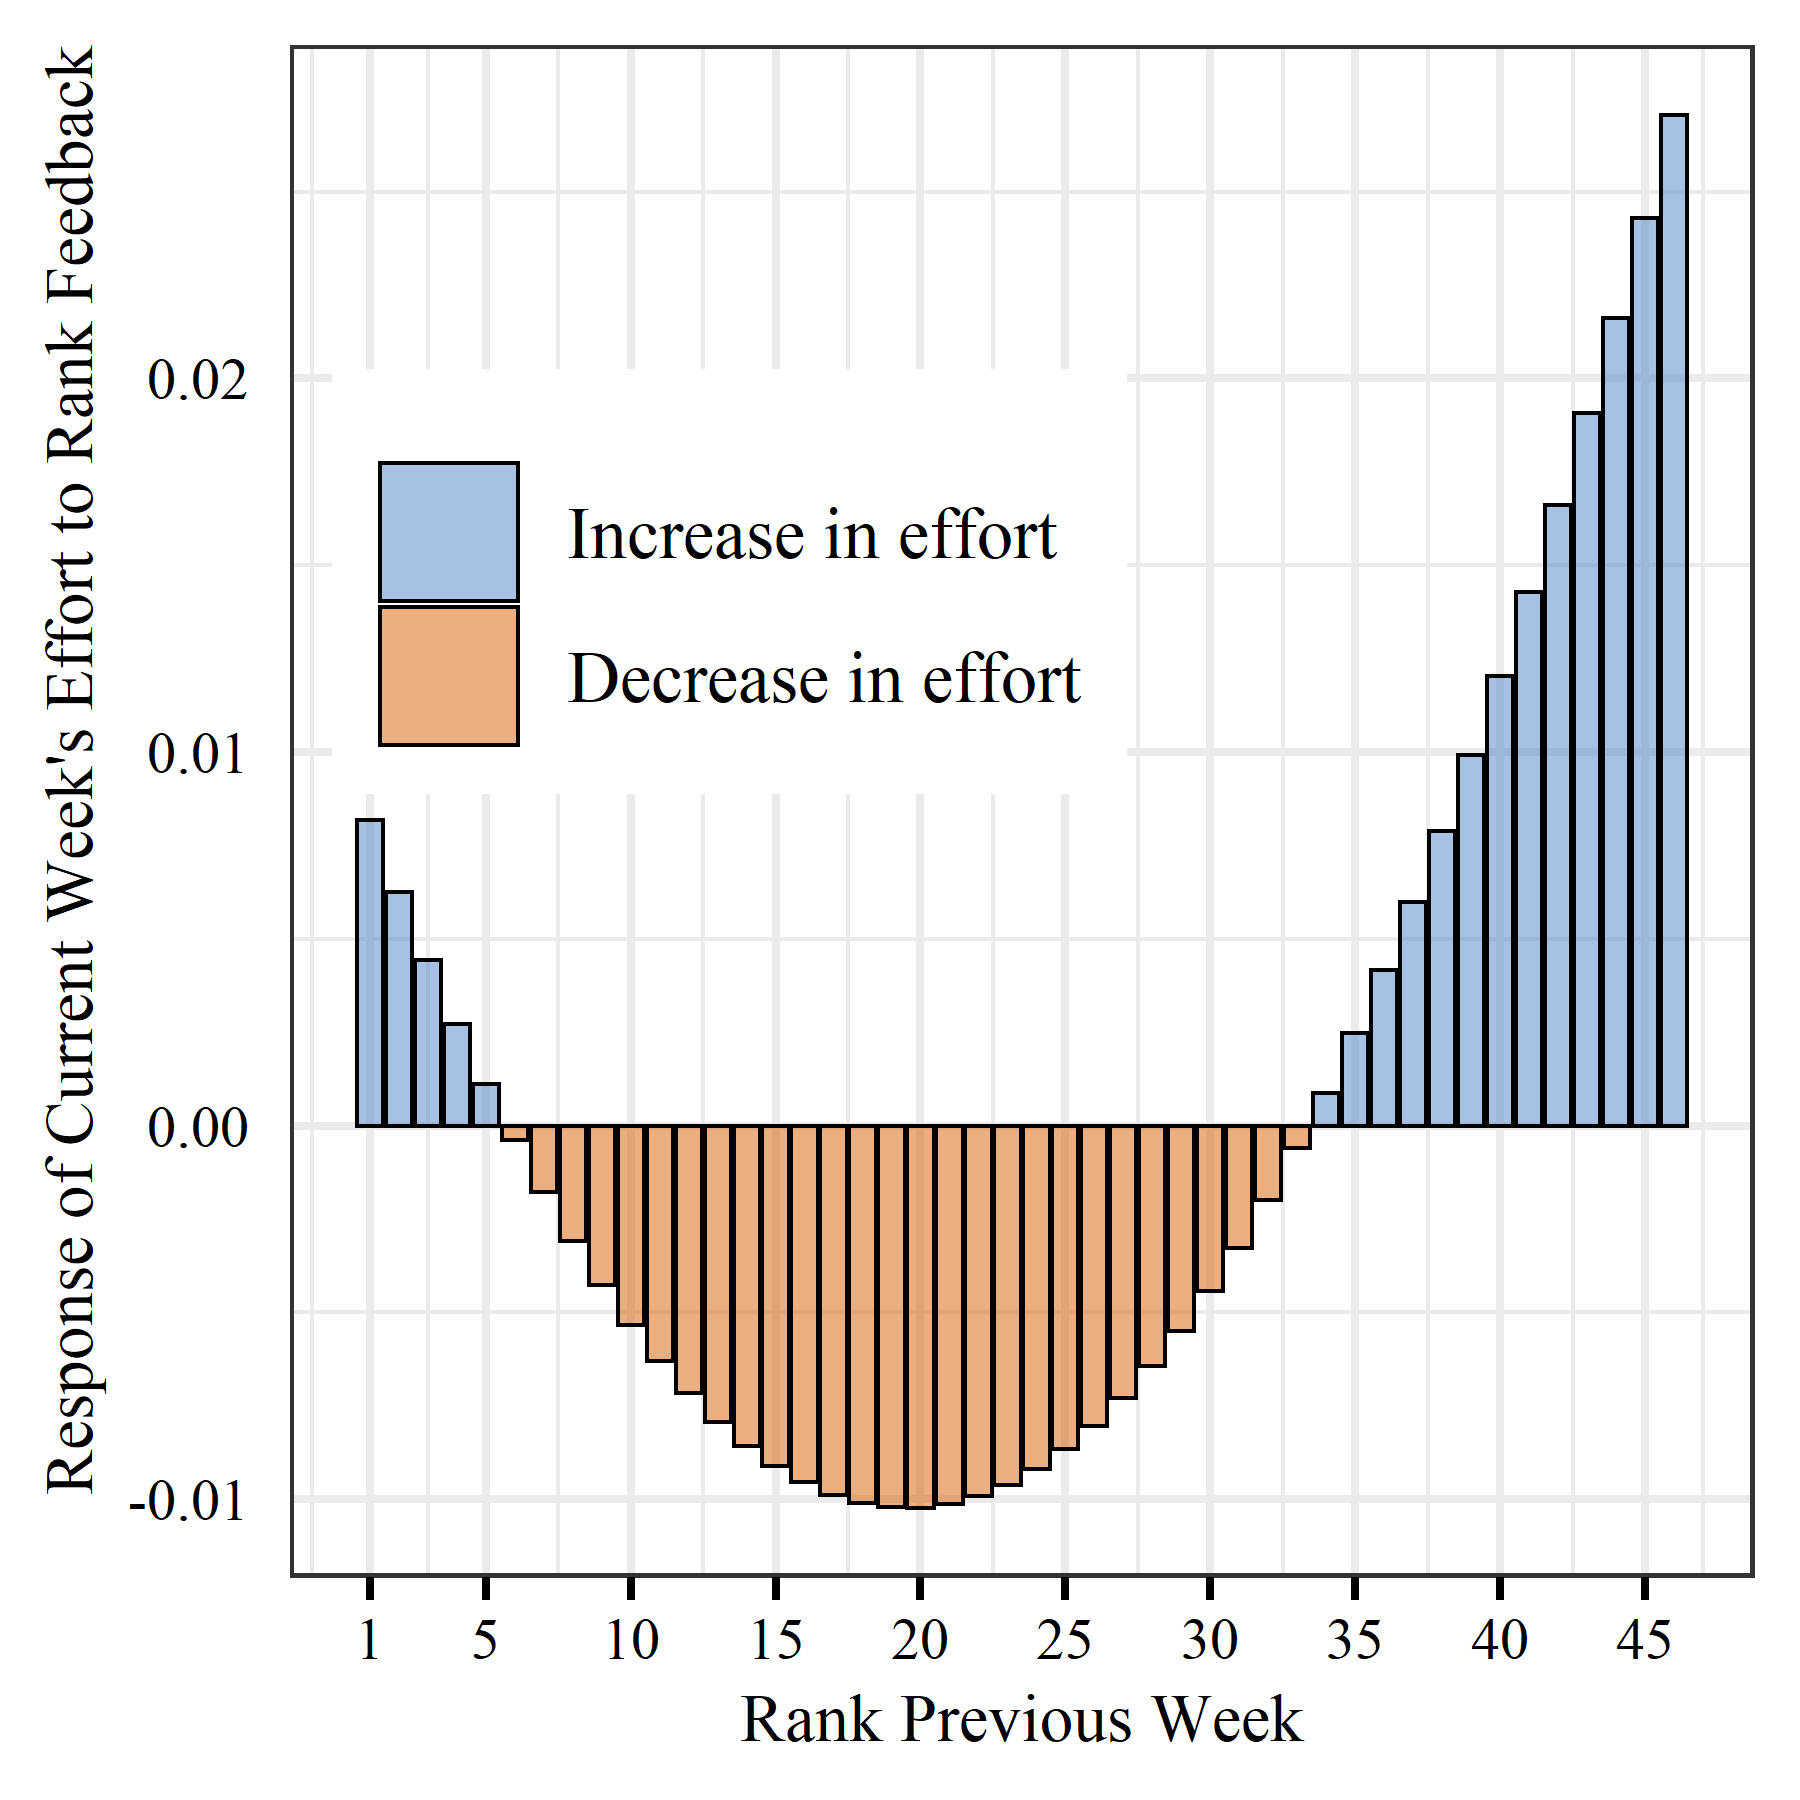
\includegraphics[scale=1]{Figures/CC/Rank Response - Ranking Group (color).png}     
     \label{fig:rank_resp}
    %  \floatfoot{\textit{Note:} These are some figure notes... }
 \end{figure} 
 
 \subsubsection{Rank Response: Definitions of First and Last Place}
 Given our clinic context, how should we define “first” or “last” place? We initially define “first place” as the top 5 ranks and define “last place” as the bottom 5 ranks to match; we then vary these definitions and test the sensitivity of our findings. More than 20\% of the clinics rotate through the bottom 5 ranks, and only 4 clinics spend a majority of the vaccination season there. On the other hand, almost 40\% of the clinics move through the top 5 ranks but only a handful of clinics spend a majority of the vaccination season in the top 5. To further clarify the presence of FPL and LPA, we evaluate the following model using a Fixed-Effects framework. The \textbf{HighRank} and \textbf{LowRank} indicators are set to 1 if the clinic receives a ranking in the top 5 or in the bottom 5 (respectively), and 0 otherwise.
 \begin{equation} \label{rank_resp_ind} %\begin{split} %\end{split} 
       WeekSPP_{it} = \pi_0 + \pi_1 \mathbbm{1}\{LowRank\}_{i,t-1} + \pi_2 \mathbbm{1}\{HighRank\}_{i,t-1} + Week_t + Clinic_i + \epsilon_{it}
 \end{equation}  
 
 We find that moving into these positions is followed by an increase in shots per patient-population by week (Table \ref{tab:rank_effect}, Column 2). A clinic which receives a low rank leads to a +2.73\% change in shots per patient-population the following week ($p < 0.01$), but a clinic given a high rank does not yield a statistically significant change ($p > 0.15$). A formal test rejects ($p < 0.05$) the null hypothesis that receiving a low rank has the same effect as receiving a high rank ($H_0: \pi_1 = \pi_2$). These results hold under various definitions of first and last place (Section \ref{app_cc_rankResp_sens}): We observe LPA – but not FPL behavior – under a wide range of definitions. 
 
 \subsubsection{Rank Response: Robustness} \label{rpf_robust}
 Given our econometric setup, we must rule out “mean reversion” as an alternative explanation for our results. Poor performance weeks could follow high performance weeks (and vice versa), either because of fluctuation in demand or a provider’s attempt to “catch up.” If this behavior coincided with changes in rank, our explanatory variables could pick up this reversion. To test for this, we artificially ranked the clinics in the Control group (with respect to each other) and the clinics in the Rebate group. We then tested for rank response behavior in these clinics, similar to a “placebo” test, since neither of these groups actually received performance feedback. A subset of these results can be seen in Table \ref{tab:rank_art} with a complete discussion in the Appendix (Section \ref{app_cc_grp_robust}). We do not see any evidence of LPA in either the Rebate or Control groups. In the end, Last-Place Aversion as we define here manifests only among the Ranking clinics, affirming our approach and eliminating the possibility of mean reversion driving our results.
 
 We also explore whether LPA degrades with time. We find the effect intensifies with time. By adding a count of the number of weeks spent near last to Specification \ref{rank_resp}, we find the effect of one extra week ranked in the bottom 5 is statistically significant ($p < 0.01$) and is approximately the same as being ranked “35 out of 46.” We also observe stronger responses to ranking information later in the vaccination season.
 
 In conclusion, we find strong evidence to support Hypothesis 4 (Last-Place Aversion) but do not find enough evidence to support Hypothesis 3 (First-Place Loving behavior). 
 
 \begin{table}
  \resizebox{.85\textwidth}{!}{ 
  \begin{threeparttable}[t]
   \centering
   \caption{Clinic Response to “Artificial” Ranks for Rebate and Control Groups}
    \begin{tabular}{lcccc}
          & (1)   & (2)   & (3)   & (4) \\
          & \textbf{WeekSPP} & \textbf{WeekSPP} & \textbf{WeekSPP} & \textbf{WeekSPP} \\
    Clinic Group & Rebate & Rebate & Control & Control \\
    Econometric Model & Specification 2 & Specification 3 & Specification 2 & Specification 3 \\
          &       &       &       &  \\
    Rank, previous week ($\lambda_1$) & 0.000867 & -     & -0.000163 & - \\
          & (0.000782) & -     & (0.000940) & - \\
    Rank$^2$, previous week ($\lambda_2$) & -1.83e-05 & -     & -4.98e-06 & - \\
          & (2.10e-05) & -     & (2.66e-05) & - \\
    Low Flag = 1 if Rank $\in$ & -     & [44,48] & -     & [42,46] \\
    Coeff.: Low Rank ($\pi_1$) & -     & -0.0121 & -     & -0.0193 \\
          & -     & (0.0164) & -     & (0.0187) \\
          &       &       &       &  \\
    Observations & 823   & 823   & 742   & 742 \\
    \# clinics & 48    & 48    & 46    & 46 \\
    \end{tabular}%
    \medskip
    \begin{tablenotes}
      \footnotesize
      \item \textbf{Table Note:} Clinic-robust standard errors in parentheses. All models include week fixed effects. 
      \item (*** $p < 0.01$, ** $p < 0.05$, + $p < 0.1$)
    \end{tablenotes}
  \label{tab:rank_art}
  \end{threeparttable} }
 \end{table}
 
 \subsection{Overall Implications of Relative Performance Feedback}
 Compliance Care 2018 led to an increase in flu shots, particularly for the group given RPF. As the season progressed, clinics might have competed for higher ranks or simply tried to avoid falling behind. But which clinics improved? Are the high performers “over-achieving”? Or have we pulled up the performance of the clinics who would generally have watched the season progress without extra effort?
 
 To answer this question, we use the artificial rankings for the Control clinics (Section \ref{rpf_robust}) to match these clinics to the Ranking clinics at the end of the season. These matched Control clinics serve as a counter-factual for the Ranking clinics had they not received RPF. Please see Figure \ref{fig:rank_v_ctrl} for reference, where higher ranks (i.e., 42-46) signify worse performance and lower ranks signify better performance. With only two exceptions, the Ranking clinics outperform their similarly ranked Control clinics. Overall, the Ranking clinics outperform their respective controls by 10.3 percentage points. The great gap emerges among the clinics with negative performance (administered fewer shots in 2018), where the Ranking clinics outperform their respective controls by 22.9 percentage points (Figure \ref{fig:rank_v_ctrl}, top left quadrant).  
 
 Thus, while relative performance feedback elevated the performance of nearly all Ranking clinics, this is particularly true for the worst performing clinics. Last-Place Aversion appears to have enticed poor performing clinics to continue to vaccinate and “stick with the program.” These results are consistent with the literature on general performance feedback \citep[e.g.,][]{Kuhnen2012,Charness2014} while also illustrating how improvement may vary depending on the specific rank or place \citep{Gill2019}. Although our rankings are anonymous, our result is similar to \cite{Song2018a} in that the poor performers gain the most from RPF. We further link this reaction to an aversion for being ranked near last, similar to \cite[p. 35]{Buell2021}: “…that the desires to get out of and to avoid falling into last place, are powerful motivators that can help drive human behavior.” We find exactly that: An aversion for last (even generally defined) drives beneficial behavior and performance improvement.
 
 \begin{figure}[htbp]
     \centering
     \caption{Performance Gap between Ranking and Control Clinics by Rank at End of Experiment} %\medskip
     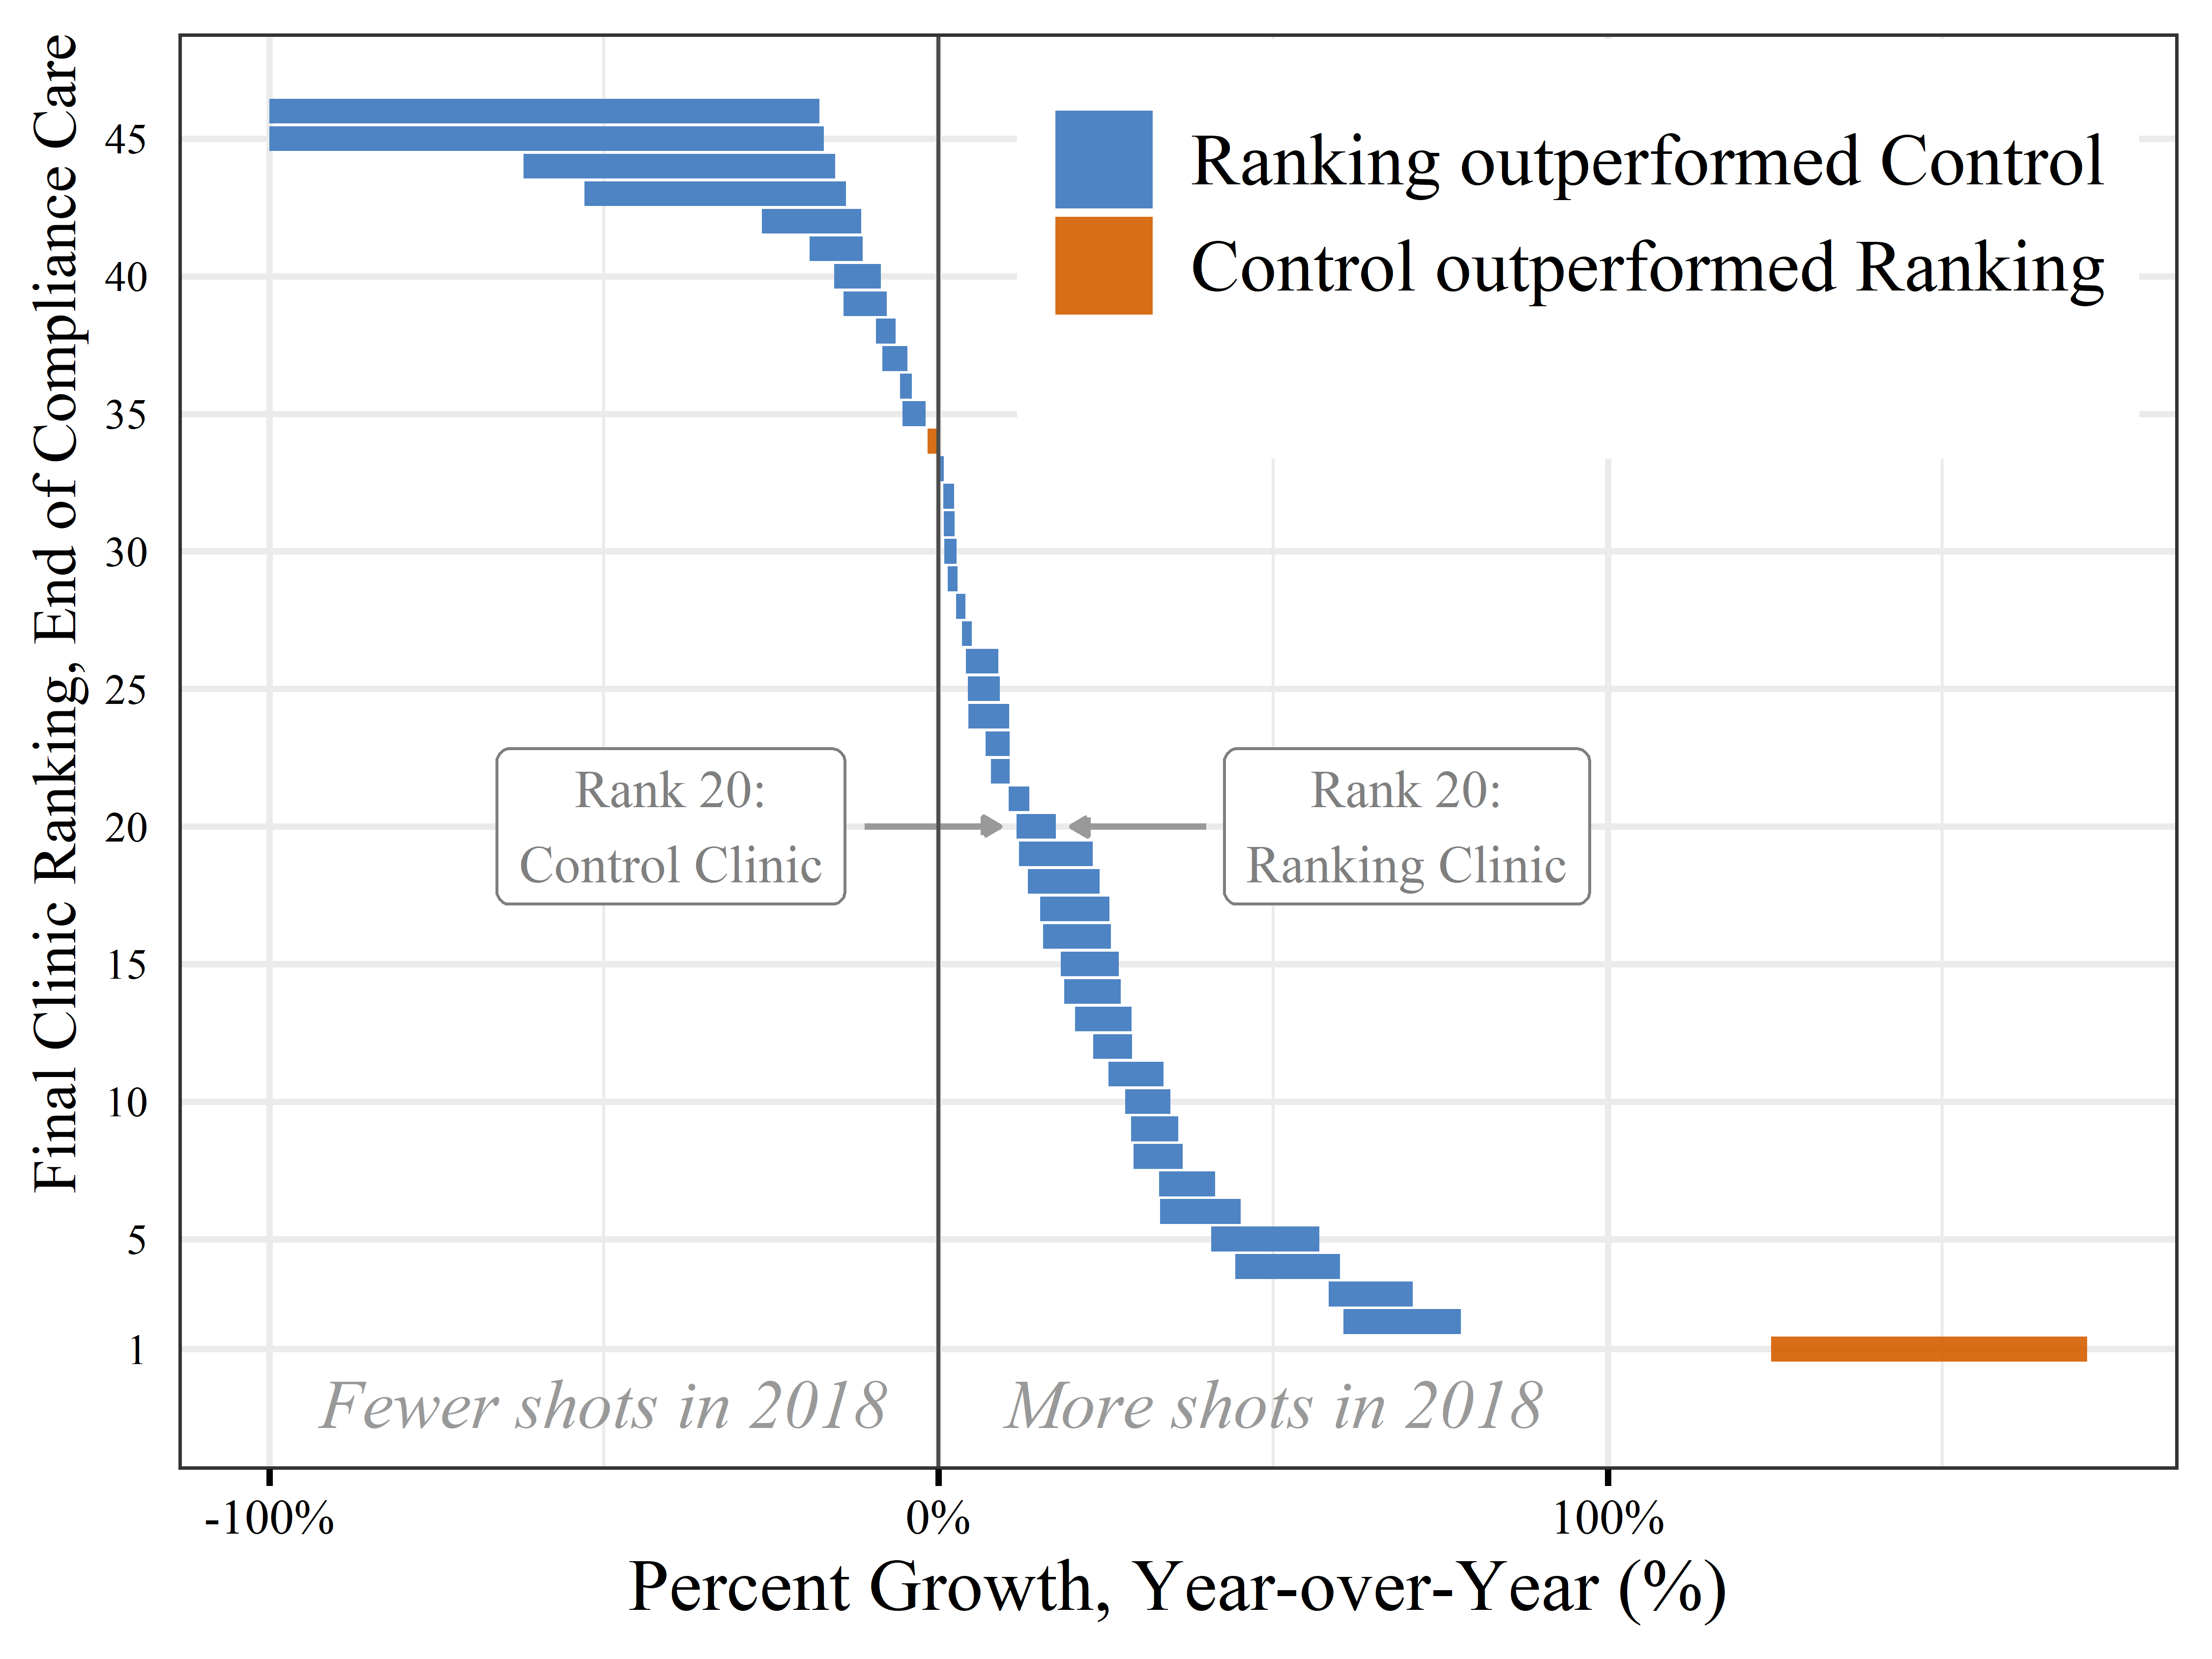
\includegraphics[scale=1]{Figures/CC/CC_RankVsControl_Fig3_color.png}     
     \label{fig:rank_v_ctrl}
     \floatfoot{\textbf{Figure Note:} This figure illustrates the clinic-to-clinic performance gap between hypothetically ranked Control clinics and the Ranking clinics at the end of Compliance Care. Larger bars indicate greater gaps. Darker shaded bars indicate ranks where the Ranking clinics outperformed Control clinics.}
 \end{figure} 


\section{Discussion \& Conclusion} \label{Conclusion_CC}
 The CDC continues to look for ways to achieve broad-scale compliance with recommended vaccination protocols, and for good reason. During the 2018-19 flu season, the CDC estimates the flu vaccine averted up to 7.1 million instances of flu-like illness and 3.8 million medical visits \citep{Chung2020}. Compliance starts with public interest: Consider that there were 4-times the number of Google searches for “flu vaccine” in August 2020 than a year prior as concerns of a Covid-19 and influenza “twindemic” escalated \citep{Google2021,NYTimes2020}. Even so, the lack of recent flu shot progress reveals a rift between vaccine interest and vaccine compliance, yielding critical implications for reducing the effects of influenza as well as the deployment of other vaccines going forward.
 
 The inherent nature of flu vaccine compliance complicates any solution since compliance requires action by two parties: Providers and patients -– the supply- and demand-side of the equation. Despite individual successes increasing demand \citep[e.g.,][]{Milkman2011}, the flu vaccination rate remains largely unchanged. But studies find most patients would accept the vaccine if their provider simply recommended it \citep{Patel2017}. And since patients still report their primary care provider as the most frequent flu vaccination channel \citep[48\%, per][]{CVSHealth2018}, we believe the greatest opportunity for large scale improvement lies in vaccine provision by providers rather than vaccine solicitation from providers. 
 
 Given this approach, Compliance Care successfully encouraged treated clinics to administer more flu shots. The program led to a 5.5 percentage point increase in flu shots for the treated over the control clinics. Clinic improvement is asymmetric, though: The Ranking clinics outperformed the Control clinics by 9.8 percentage points, while the Rebate clinics only outperformed the Control clinics by 0.9 percentage points. We claim that Last-Place Aversion meaningfully drives this outcome: Despite their low ranking, the gap between the Ranking and Control clinics widened over the season such that, in the end, the worst performing Ranking clinics outperformed their respective Control clinics by 22.9 percentage points. Our supply-side approach: (1) cued attention to flu shots with (2) a near-costless intervention while still (3) preserving provider discretion by intervening at the clinic-level. Our results hold promise for addressing the broader flu vaccination problem in an effective and cost-considerate manner.
 
 Our paper makes several contributions to the literature. First, we highlight the motivational power of social comparison \citep{Festinger1954}, even over and above economic incentives. In our context, performance feedback dominates the effect of additional financial incentives. However, our experiment is limited in that we only compare one form of financial incentive to one form of RPF. To explore this, we worked with VaxCare to distribute a survey to clinics after the study ended. Among the rebate clinic respondents, 75\% indicated the incentive amount was meaningful – so we do not believe the size of the incentive was driving our result. Future work could compare different incentive systems and even explore a combination of incentives and feedback. Even so, our counter-intuitive result highlights an opportunity to leverage low-cost interventions to effectively focus healthcare provider attention on an issue of interest. 
 
 Second, when considering the clinic rankings and the role of RPF, we also find evidence of Last-Place Aversion, similar to \cite{Kuziemko2014,Gill2019} and \cite{Buell2021}. To the best of our knowledge, our analysis is the first to examine rank response behaviors in productivity among firms in a dynamic, real-world setting. Specifically, Last-Place Aversion manifests not only in individuals, but also among firms. Furthermore, the strongest effect appears among the worst performing Ranking clinics. 

 This finding comes with one limitation: Our field experiment and subsequent identification of a response does not permit us to identify the mechanism behind the response. We have demonstrated the efficacy of financial incentives and performance feedback, but some of the reasons underlying the outcomes remain untested. These reasons include exploring what specific behavior the incentive did not affect or why a clinic exhibits Last-Place Aversion or whether these behavioral changes might persist over time. Other possible mechanisms include clinics fearing repercussions of low rankings or providers perceiving the clinics as reaping the financial benefits of their individual effort. Future work should seek to clarify the processes of behavior change as well as exploring the time-sensitive nature of these behaviors (e.g., “Does Last-Place Aversion diminish over time?”). 

 Third, we contribute to the growing body of work in operations that finds an important role for discretion in driving operational performance \citep[e.g.,][]{VanDonselaar2010,Campbell2011,Kim2015,Phillips2015,Ibanez2017,Song2018a}. Vaccination rate information given to clinics then successfully diffused to front-line workers. Thus, performance feedback, even when given at a higher, firm-level, encouraged the productive use of individual discretion to improve operational performance. Few studies examine firm-level response to feedback and incentives; even fewer compare the two. Our approach fills both gaps by cueing provider attention to administer more flu shots.

 This approach raises two follow-on thoughts. First, the focusing of attention on flu shots inherently begs the question of where providers are paying less attention as a result. We are limited from seeing how other elements of patient health were affected. Despite this, because we intervene at the clinic level, we mitigate the concerns of “alert-fatigue,” which has already been shown to negatively impact patient outcomes. Instead, we allow providers full discretion in their final choice of patient care and we trust these individuals to make the best decisions for their patients. Second, given our findings, one might hypothesize about the benefits of a dual supply- and demand-side approach to vaccination compliance, as in \cite{Zimmerman2014}. Indeed, our findings clarify which elements of these more complicated approaches meaningfully alter vaccination outcomes. Future research should build on our work by combining effective supply-side cues with proven demand-side strategies, such as patient reminders.

 Finally, as a general contribution, we demonstrate the importance of running field experiments when addressing complicated operational questions \citep{Ibanez2019a}. Field experiments possess explanatory power and identification advantages which can augment archival data methods to generate both rigorous and relevant research. Given our experimental design, our results will likely generalize to other contexts: Consider that the above behaviors manifest in a randomized setting with many independent, geographically dispersed clinics despite heterogeneity in location, clinic size, and performance. Even so, we acknowledge that the clinics in this study represent VaxCare partners that consented to join the experiment. Future work should continue to study these topics in other industries and explore whether incentives or performance feedback lead to differing rates of intervention attrition.
 
 One limitation exists surrounding our experimental design. After recruitment, no further action was taken with the Control group; this setup most accurately replicates the real-world setting for a VaxCare partner. Because of this, the possibility remains for an email “reminder” effect for the treated clinics. This effect seems unlikely – as the Rebate clinics receive emails and still do not statistically outperform the Control clinics – but we recognize the inherent limitation of our clinical context. 
 
 Our findings have a number of managerial implications. First, although many organizational interventions lead to performance improvement, Compliance Care achieved improvement in a domain bereft of significant improvement in more than a decade with minimal cost. As mentioned before, even a 1 percentage point increase in vaccine coverage could yield significant societal benefits. If half of these shots went to seniors – a higher risk age group – CDC reports estimate this would prevent more than 2500 hospitalizations \citep{Rolfes2019}. Furthermore, the effects of RPF are “long-lasting” \citep{Blanes-i-Vidal2011} and persistent \citep{Delfgaauw2013}. Thus, we expect enduring benefits from any positive outcome, even under financial constraints. Furthermore, policy makers can leverage other operations literature to scale our intervention \citep{Drakopoulos2017, Gupta2020}.
 
 Second, we note that operational structure helps to selectively focus decision makers’ attention. Small attention cues can encourage decision makers in any organizational context to selectively focus their attention on important tasks \citep[e.g.,][]{Song2018a,Kim2020}. Finally, we must note that one cannot cue attention to all desired behaviors. The introduction of multiple cues would likely reduce the effectiveness of each cue with a potentially worse end state. We caution managers to be mindful of their use and to prioritize interventions which achieve the greatest benefit via the smallest impact.
 
 We conclude appropriate supply-side behavioral intervention programs can improve performance, even when targeting seemingly immutable trends, such as influenza vaccination rates. Our results show promise for improvements in public health and more generally for company operations.
 
%  \end{onehalfspace}
 
 